\chapter{Une méthode de composition dynamique des services Web
  sémantiques utilisant Neo4j}
\label{ch:approach}

\section*{Introduction}
\addcontentsline{toc}{section}{Introduction} \markboth{INTRODUCTION}{}

\newpage
\section{Définitions préliminaires}
\label{sec:basic-defs}
Cette section a comme but d'introduire les notions de base ainsi que
les notations et terminologies \ref{sec:basic:ws} employées dans la
suite de ce chapitre. Nous présentons une formulation
mathématique de notre problème principal, à savoir \textit{la
  composition des servies Web} sous forme d'un problème de recherche
du plus court chemin dans un graphe orienté
\ref{sec:basic:composition}.\medskip

\subsection{Services Web}
\label{sec:basic:ws}

Chaque service web peut contenir les définitions de différentes
opérations \acrshort{wsdl} identifiables par leurs noms et leurs
paramètres. Pour des raisons de simplicité, nous supposons que chaque
service Web représente une seule opération.\medskip

\begin{mydef}[\textbf{Service Web}]
  Un Service Web $S$ est un 2-tuple $\mathpzc{<I,O>}$, où
  $\mathpzc{I}=\{I_0, \dots, I_n\}$ désigne l'ensemble des paramètres
  d'entrées, $\mathpzc{O}=\{O_0, \dots, O_m\}$ l'ensemble des
  paramètres de sorties.
\end{mydef}

%!TEX root = ../../main.tex
\begin{figure}[h]
    \centering
    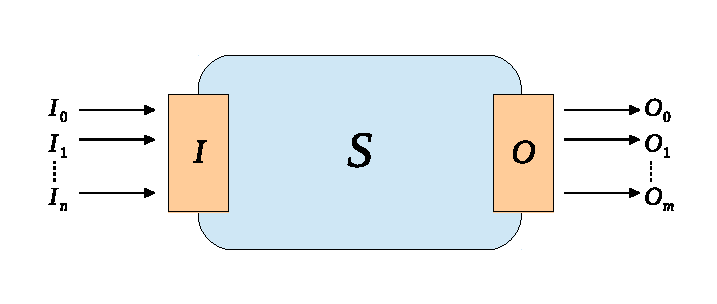
\includegraphics[width=0.65\textwidth]{figs/ch3/ws.eps}
    \caption{Un service Web atomique.}
    \label{fig:ch3/ws}
\end{figure}
%%% Local Variables:
%%% mode: latex
%%% TeX-master: "../../main"
%%% End:


Dans notre approche proposée, nous supposons que chaque service est
décrit par un document \acrshort{owls} qui possède un seule processus
atomique, et que chaque paramètre est lié à un concept dans
l'ontologie \acrshort{owl} du domaine.\medskip

\begin{mydef}[\textbf{Annuaire des services Web}]
  un annuaire des services Web est un ensemble
  $\mathpzc{R} =\{\mathpzc{S}_0, \mathpzc{S}_1, \dots,\mathpzc{S}_n\}$
  des services Web disponibles, où chaque
  $\mathpzc{S} \in \mathpzc{R}$ est un service Web.
\end{mydef}

%!TEX root = ../../main.tex
\begin{figure}[h]
    \centering
    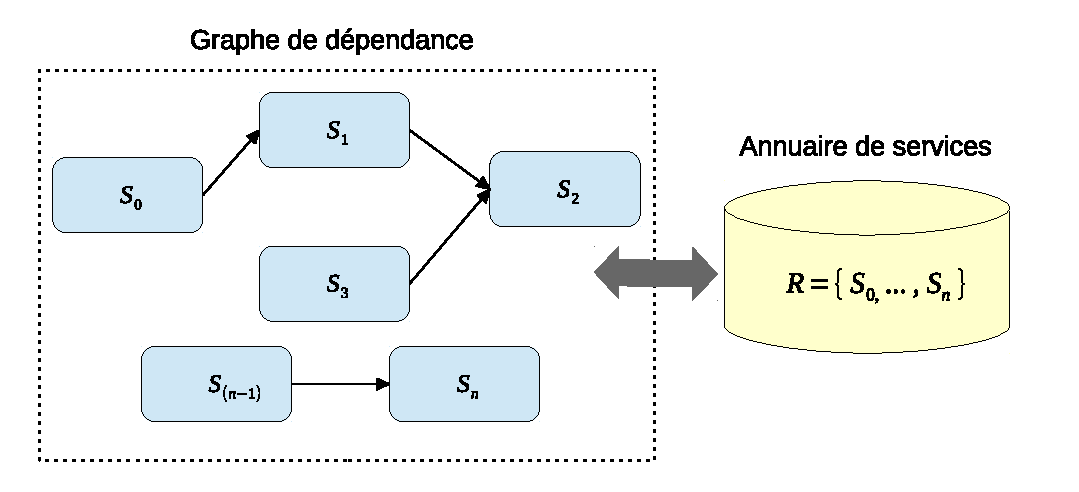
\includegraphics[width=1.1\textwidth]{figs/ch3/gd.eps}
    \caption{Graphe de dépendance $\mathpzc{GD}$ entre les services
      Web d'un annuaire $\mathpzc{R}$.}
    \label{fig:ch4/gd}
\end{figure}
%%% Local Variables:
%%% mode: latex
%%% TeX-master: "../../main"
%%% End:


\subsection{Composition de services Web}
\label{sec:basic:composition}
Afin de découvrir et sélectionner un service Web composite suite à
une requête du client de composition, les services référencés dans un
annuaire doivent être structurés dans un graphe orienté modélisant
  toutes les relations de dépendance fonctionnelle possibles pour permettre
  de réaliser un \textit{Matching} horizontal \ref{sec:ch4/matching}
  (la figure \ref{fig:ch4/gd}) entre les services disponibles deux à deux.\medskip

  \begin{mydef}[\textbf{Graphe de dépendance}]
    Un graphe de dépendance $GD$ est un ``graphe orienté et
    acyclique'' $GD=<R, E_r>$ qui modélise toutes les relations de
    dépendance fonctionnelle possibles entre les services Web
    disponibles dans un annuaire $R$. Il existe une relation $e=(s_0,
    s_1) \in E_r$ si et seulement si il existe une relation de
    dépendance entre $s_0$ et $s_1$.
  \end{mydef}

  L'approche proposée consiste à construire le graphe de dépendance à
  priori (\textit{Offline}) et le sauvegarder dans une base de données
  graphe (\textit{Neo4j}). Suite à une requête $Q$, un sous-graphe $G$
  est extrait reflétant un plan de composition exécutable $P$ d'un
  service Web composite satisfaisant.

  \begin{mydef}[\textbf{Requête}]
    Une requête $Q$ est un tuple $Q = <I', O'>$. $I'$ désigne la liste
    des paramètres d'entrée fournis par le client et $O'$ représente
    la listes des paramètres requis (sorties).
  \end{mydef}

  %!TEX root = ../../main.tex
\begin{figure}[h]
    \centering
    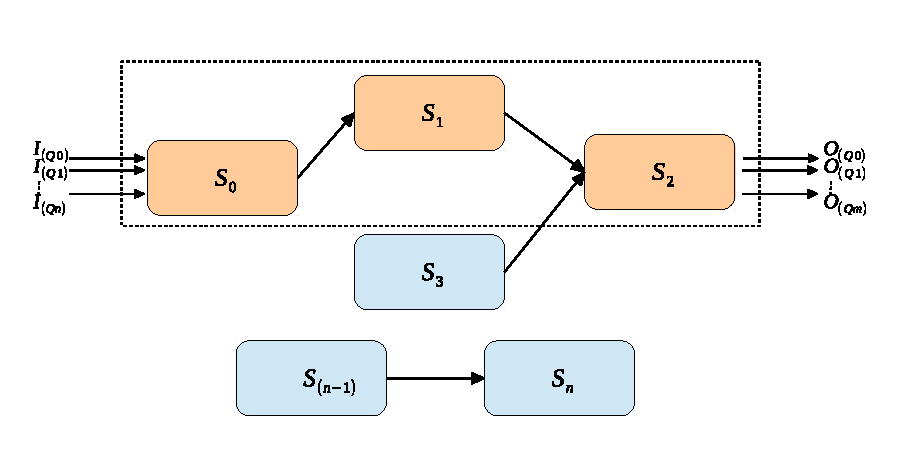
\includegraphics[width=1\textwidth]{figs/ch3/composition-plan.eps}
    \caption{Un service Web composite avec le plan de composition correspond.}
    \label{fig:ch3/composition-plan}
\end{figure}
%%% Local Variables:
%%% mode: latex
%%% TeX-master: "../../main"
%%% End:


  \begin{mydef}[\textbf{Plan de composition}]
    Un plan de composition $P$ est un sous-graphe
    $G$``\textbf{connexe''} d'un graphe de dépendance $GD$, $G=(V,E)$
    tel que $G \subset GD$ décrit le flux de données/contrôles
    d'exécution d'un ensemble de services Web atomiques $V \subset R$
    engagés dans un processus de composition. Il existe une arête $e
    \in E$ tel que $e = (s_i, s_j)$ si l'exécution d'un service $s_j$
    dépend d'un ou plusieurs paramètres de sortie de $s_i$.
  \end{mydef}

  \begin{mydef}[\textbf{Service Web composite}]
    Un service Web composite $S_c$ est un service Web exécutable
    composé de ``$n$'' services atomiques $s \in \{s_0,..., s_n\}$ tel
    que $n \succeq 1$, l'exécution d'un service Web composite
    correspond à l'exécution d'un plan de composition $P$ décrit par
    $G=<V,E>$ où $V = \{s_0, ..., s_n\}$ et $E$ décrivent les
    relations de dépendance entre les services $V$.
  \end{mydef}

  La figure \ref{fig:ch4/composition-plan} montre un service Web
  composite $S_c = <\{i_0, i_1\}, \{o_0, o_1\}>$ correspondant à un
  plan de composition $P$ représenté par un graphe\\ $G =<\{s_0, s_1,
  s_2, s_4\}, \{(s_0, s_1), (s_1, s_2), (s_2, s_4)\}>$.

\section{Architecture proposée}
\label{sec:proposition}

\section{Matching des services  atomiques}
\label{sec:ch4/matching}

\section{Construction et persistance du graphe de dépendance dans une
  base de données Neo4J}
\section{Découverte et exécution des services composites}

\section*{Conclusion}
\label{sec:conclusion}
\addcontentsline{toc}{section}{Conclusion} \markboth{CONCLUSION}{}


%%% Local Variables:
%%% mode: latex
%%% TeX-master: "../main"
%%% End:
